

\documentclass{beamer}

\mode<presentation> {

  % The Beamer class comes with a number of default slide themes
  % which change the colors and layouts of slides. Below this is a list
  % of all the themes, uncomment each in turn to see what they look like.

  % \usetheme{default}
  % \usetheme{AnnArbor}
  % \usetheme{Antibes}
  % \usetheme{Bergen}
  % \usetheme{Berkeley}
  % \usetheme{Berlin}
  % \usetheme{Boadilla}
  % \usetheme{CambridgeUS}
  % \usetheme{Copenhagen}
  % \usetheme{Darmstadt}
  % \usetheme{Dresden}
  % \usetheme{Frankfurt}
  % \usetheme{Goettingen}
  % \usetheme{Hannover}
  % \usetheme{Ilmenau}
  % \usetheme{JuanLesPins}
  % \usetheme{Luebeck}
  \usetheme{Madrid}
  % \usetheme{Malmoe}
  % \usetheme{Marburg}
  % \usetheme{Montpellier}
  % \usetheme{PaloAlto}
  % \usetheme{Pittsburgh}
  % \usetheme{Rochester}
  % \usetheme{Singapore}
  % \usetheme{Szeged}
  % \usetheme{Warsaw}

  % As well as themes, the Beamer class has a number of color themes
  % for any slide theme. Uncomment each of these in turn to see how it
  % changes the colors of your current slide theme.

  % \usecolortheme{albatross}
  \usecolortheme{beaver}
  % \usecolortheme{beetle}
  % \usecolortheme{crane}
  % \usecolortheme{dolphin}
  % \usecolortheme{dove}
  % \usecolortheme{fly}
  % \usecolortheme{lily}
  % \usecolortheme{orchid}
  % \usecolortheme{rose}
  % \usecolortheme{seagull}
  % \usecolortheme{seahorse} 
  % \usecolortheme{whale}
  % \usecolortheme{wolverine}

  % \setbeamertemplate{footline} % To remove the footer line in all slides uncomment this line
  % \setbeamertemplate{footline}[page number] % To replace the footer line in all slides with a simple slide count uncomment this line

 % \setbeamertemplate{navigation symbols}{} % To remove the navigation symbols from the bottom of all slides uncomment this line
}
\usepackage{amsmath}
\usepackage{graphicx} % Allows including images
\usepackage{booktabs} % Allows the use of \toprule, \midrule and \bottomrule in tables
\usepackage{tikz}
\newcommand\mysim{\mathrel{\overset{\makebox[0pt]{\mbox{\normalfont\tiny\sffamily iid}}}{\sim}}}
\def\checkmark{\tikz\fill[scale=0.4](0,.35) -- (.25,0) -- (1,.7) -- (.25,.15) -- cycle;} 

% ----------------------------------------------------------------------------------------
%	TITLE PAGE
% ----------------------------------------------------------------------------------------

\title[ABC]{Introduction to Approximate Bayesian Computation} % The short title appears at the bottom of every slide, the full title is only on the title page

\author{John Haman} % Your name
\institute[BGSU] % Your institution as it will appear on the bottom of every slide, may be shorthand to save space
{
  Bowling Green State University \\ % Your institution for the title page
  \medskip
  \textit{jthaman@bgsu.edu} % Your email address
}


\date{\today} % Date, can be changed to a custom date

\begin{document}

\begin{frame}
  \titlepage % Print the title page as the first slide
\end{frame}


% ----------------------------------------------------------------------------------------
%	PRESENTATION SLIDES
% ----------------------------------------------------------------------------------------
\begin{frame}
  \frametitle{Implicit models}

Two types of statistical models:

\begin{itemize}
\item Prescribed models - Likelihood function is available, common for us
\item Implicit models - mechanisms for simulating data, common for biologists, psychologist

\pause
\vskip 0.5in

Implicit models give scientists more freedom to model phenomena, complex processes are favored over simple ones
\end{itemize}

\end{frame}

\begin{frame}
  \frametitle{Monte Carlo inference}

Aim to sample from a posterior distribution:

$$  \pi ( \theta | \mathcal{D} ) \propto \mathbb{P}( \mathcal{D} | \theta) * \pi ( \theta) $$ 
\pause
MCMC is great for performing Bayesian inference in complex models, and it's exact up to a monte carlo error. It's not great when.... 

\pause

\begin{itemize}
\item $\mathbb{P} (\mathcal{D} | \theta) $ is unknown or intractable. 
\pause
\item independence cannot be assumed for many model parameters
\end{itemize}

So there is a need for generating posterior data without a likelihood function
\end{frame}


\begin{frame}
  \frametitle{Likelihood free inference}

\begin{block}{Rejection Algorithm (old way)}
  \begin{itemize}
  \item Draw $\theta$ from $\pi(*)$
  
  \item Accept $\theta$ with probability $\mathbb{P} (\mathcal{D} |\theta)$
  \end{itemize}
\pause
\end{block}
\pause
\begin{block}{Mechanical Rejection Algorithm (Without Likelihood)}

  \begin{itemize}
  \item Draw $\theta$ from $\pi(*)$
    
  \item Simulate $\mathcal{D}' \sim \mathbb{P} ( * | \theta)$

  \item Accept $\theta$ if $\mathcal{D} = \mathcal{D}'$
  \end{itemize}
\end{block}

The last requirement is probably too restrictive, e.g. if the data are continuous
 
\end{frame}

\begin{frame}
  \frametitle{ABC}

  \begin{block}{ABC Rejection}
    \begin{itemize}
  \item Draw $\theta$ from $\pi(\theta)$

    
  \item Simulate $\mathcal{D}' \sim \mathbb{P} (* | \theta)$

  \item Accept $\theta$ if $d ( \mathcal{D} , \mathcal{D}' ) < \epsilon$, or if
    $d ( S( \mathcal{D} ), S(\mathcal{D}') ) < \epsilon$, $S$ is a sufficient statistic. 
  \end{itemize}
\end{block}
\pause

This generates data from is distribution $ \pi (\theta | d ( \mathcal{D} , \mathcal{D}' ) < \epsilon) $

\begin{itemize}
\item  If $\epsilon \to 0$, we obtain data from the target density, $\pi(\theta | \mathcal{D})$.
\item If $\epsilon \to \infty$ we obtain data from the prior, $\pi(\theta)$.

\end{itemize}

\pause

Many types of ABC algorithms now... M-H, regression based, neural networks, all implemented by the \texttt{R} package \texttt{abc}.

\end{frame}


\begin{frame}
  \frametitle{Metropolis Hastings}

Rejection sampling is very inefficient, because $\theta $ is being sampled from the prior at each step

\pause

We can speed things up by correlating observations to spend more time in regions of high likelihood...

\begin{block}{Metropolis-Hastings with ABC}

  \begin{itemize}
  \item Suppose we are at $\theta$. Propose $\theta'$ from density $q ( \theta, \theta')$
  \item Simulate $\mathcal{D}'$ from $\mathbb{P} ( * | \theta')$
  \item  If $ d ( \mathcal{D}, \mathcal{D}') \leq \epsilon $ calculate 

    $$ h ( \theta , \theta ' ) = \min \left( 1 , \frac{ \pi(\theta') q ( \theta' , \theta)}{ \pi(\theta) q ( \theta, \theta')} \right)$$
  \item  Accept the move to $\theta'$ with probability $h( \theta, \theta')$, else stay at $\theta$.
  \end{itemize}
  
\end{block}

\end{frame}


\begin{frame}
  \frametitle{Example}

  \begin{block}{Normal data}
    \begin{itemize}
    \item Generate $\mathcal{D} \sim N(5.3 , 2.7^2)$ Save $\bar{\mathcal{D}}$ and $sd(\mathcal{D})$.
    \item Accept $\mathcal{D}'$ if $ d ( \bar{\mathcal{D}'} , \bar{\mathcal{D}}) < 0.1 $ and $ d (sd(\mathcal{D}') , sd ( \mathcal{D} )) < 0.2$. 
    \item Initialize MH algorithm
      
    \item  Add parameters that generated $\mathcal{D}'$ to chain with probability $h$ if $\mathcal{D}'$ is accepted.
    \end{itemize}
  \end{block}

\end{frame}

\begin{frame}
  \begin{center}
    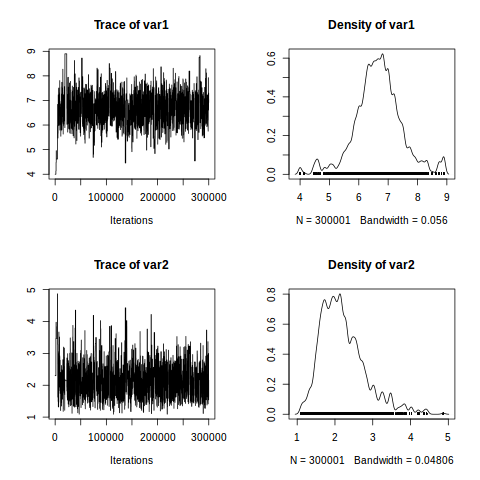
\includegraphics[scale=0.4]{posterior.png}

Trace and marginal distributions of the posterior sample. 
  \end{center}
\end{frame}
\end{document} 